% !TEX root = main.tex

\section{内存管理}
\subsection{分区存储管理}
固定分区
\begin{itemize}
    \item 等长分区:大进程则只能部分载入,小进程将产生内碎片
    \item 不等长分区:一定程度上缓解等长分区的问题
\end{itemize}

动态分区:会存在外碎片;若采用压缩方式移动进程使其紧靠,则非常耗时,需要进行动态重定位
\begin{figure}[H]
    \centering
    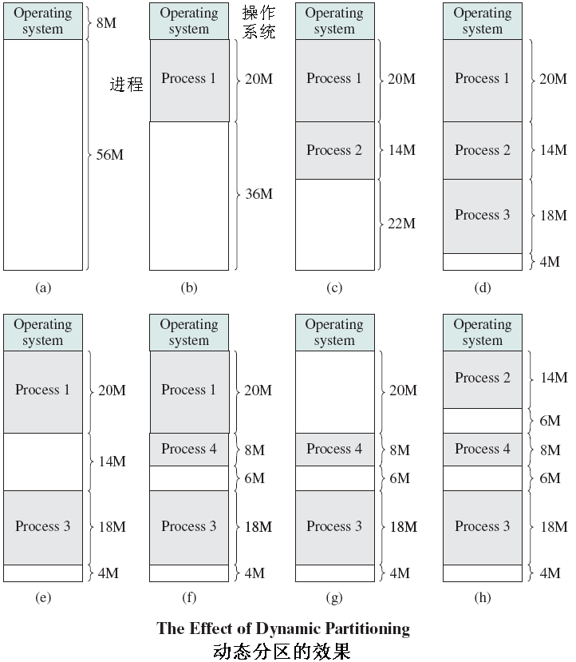
\includegraphics[width=0.6\linewidth]{fig/dynamic_partition.png}
\end{figure}

动态分区放置算法:
\begin{itemize}
    \item 首次适配(first fit):从前端开始扫描内存,直到找到一个足够大的空闲区,通常性能比较好
    \item 下次适配/邻近适配(next fit):从上次分配结束的地方开始扫描内存,直到找到一个足够大的空闲区
    \item 最佳适配(best fit)算法:扫描整个内存,找出一个足够大的最小的空闲区,会产生很多外部碎片
\end{itemize}

伙伴系统(buddy system):固定分区和动态分区的折中方案
\begin{itemize}
    \item 可用内存块大小为$2^K,L\leq K\leq U$
    \item 初始空间大小为$2^U$
    \item 若请求空间大小$s<2^{U-1}$,则对分现有块
\end{itemize}

\begin{figure}[H]
    \centering
    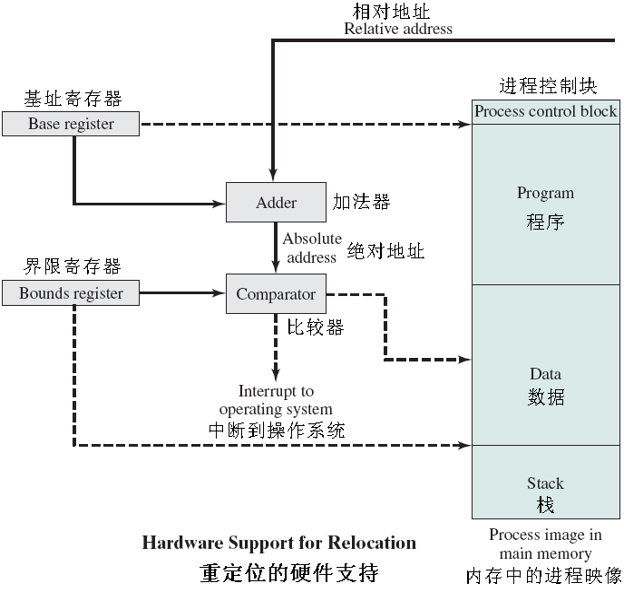
\includegraphics[width=0.5\linewidth]{fig/relocation.png}
    \caption*{重定位的硬件机制}
\end{figure}

\subsection{页式存储管理}
分页(paging)
\begin{itemize}
    \item 将主存划分为许多等长的帧/页框(frame)
    \item 将进程划分为若干页(page)
    \item 进程加载时,所有页面被载入可用帧,同时建立页表
\end{itemize}

设页大小为$L$,逻辑地址$A$,物理地址$E$,则
\[\text{页号}P=A/L\qquad\text{页内偏移量}W=A\%L\]

\begin{example}
    16位编址,若页面大小为1K(1024),则需(低)10位表示页内偏移,剩下(高)6位表示页号,则
    \begin{itemize}
        \item 相对地址为$1502$的逻辑地址$ = 1024 + 478 = (1, 478)$
        \item 逻辑地址为$(1, 478)$的相对地址$ = 1*1024 + 478 = 1502$
    \end{itemize}
\end{example}

类似固定分区,不同在于:
\begin{itemize}
    \item 分页中的“分区”(页帧)非常小(从而内碎片也小)
    \item 分页中一个进程可占用多个“分区” (页帧)(从而不需要覆盖)
    \item 分页中不要求一个进程占用的多个“分区”(页帧)连续(充分利用空闲“分区”)
\end{itemize}
存在问题:
\begin{itemize}
\item 不易实现共享和保护(不反映程序的逻辑组织)
\item 不便于动态链接(线性地址空间)
\item 不易处理数据结构的动态增长(线性地址空间)
\end{itemize}

\subsection{段式存储管理}
将程序及数据划分成若干段(segment)(不要求等长,但不能超过最大长度)
\begin{itemize}
    \item 分页是出于系统管理的需要,分段是出于用户应用的需要:
    一条指令或一个操作数可能会跨越两个页的分界处,而不会跨越两个段的分界处
    \item 页大小是系统固定的,而段大小则通常不固定
    \item 逻辑地址表示
    \begin{itemize}
    \item 分页是一维的,各个模块在链接时必须组织成同一个地址空间
    \item 分段是二维的,各个模块在链接时可以每个段组织成一个地址空间
    \end{itemize}
    \item 通常段比页大,因而段表比页表短,可以缩短查找时间,提高访问速度
    \item 分段对程序员可见,从而可用来对程序和数据进行模块化组织
    \item 分段方便实现模块化共享和保护,如程序可执行、数据可读写(段表表项要有保护位)
    \item 都存在外碎片,但分段中可通过减少段长来减轻外碎片浪费程度
    \item 分段中一个进程可占用多个“分区” ,不要求一个进程占用的多个“分区”连续(但一般要求一个段所占用的多个“分区”连续)
    \item 分段克服了分页存在的问题(数据结构的动态增长、动态链接、保护和共享)
    \item 分段存在外碎片,分页只有小的内碎片,分页内存利用率比分段高
\end{itemize}

段表只能有一个,而页表可以有多个。

段页式系统中,逻辑地址被分为段号S、页号P和页内偏移量W。

逻辑地址偏移量只需小于段的长度即可。

\subsection{虚拟存储}
传统的存储方式都是一次性加载,并且驻留在内存中。
而虚拟存储器则是基于程序的局部性原理,在程序装入时,将程序一部分装入内存,其余部分留在外存。
\begin{itemize}
    \item 采用部分加载,内存中可同时容纳更多的进程。
每个进程都只加载一部分,更多进程中应该也会有更多的就绪进程,从而提高CPU利用率
    \item 采用部分加载,进程可以比内存大,实现了虚拟存储
    \begin{itemize}
\item 用户程序可以使用的独立于物理内存的逻辑地址单元组成存储空间(虚拟存储)
\item 逻辑地址空间可以比物理地址空间大,例如,设物理内存64KB,1KB/页,则物理地址需要16位,而逻辑地址可以是28位!
\item 虚拟存储由内存和外存结合实现
    \end{itemize}
\end{itemize}

虚拟存储技术的特征:不连续性、部分交换、大空间

抖动(thrashing)问题:交换操作太过频繁

页表
\begin{itemize}
\item 页表项(Page Table Entry,简称为PTE)的一般内容:
\begin{itemize}
\item Present:在/不在内存
\item Modified:有没有被修改
\item Protection:保护码,1位或多位(rwe:读/写/执行)
\item Referenced:有没有被访问
\item Cache:是否禁止缓存
\end{itemize}
\item 页表长度不定,取决于进程大小
\item 不适合用寄存器存储页表,而是存放在内存
\item 页表起始地址保存在一个CPU专用寄存器里(\verb'cr3')
\end{itemize}

虚拟地址转换为物理地址流程:
\begin{itemize}
    \item 将虚拟地址分割为虚页号和偏移量两个部分
    \item 通过虚页号在页表中寻找对应的表项
    \item 从中获取页框号后,乘页尺寸,加上偏移量,得到物理地址
\end{itemize}

\begin{figure}[H]
    \centering
    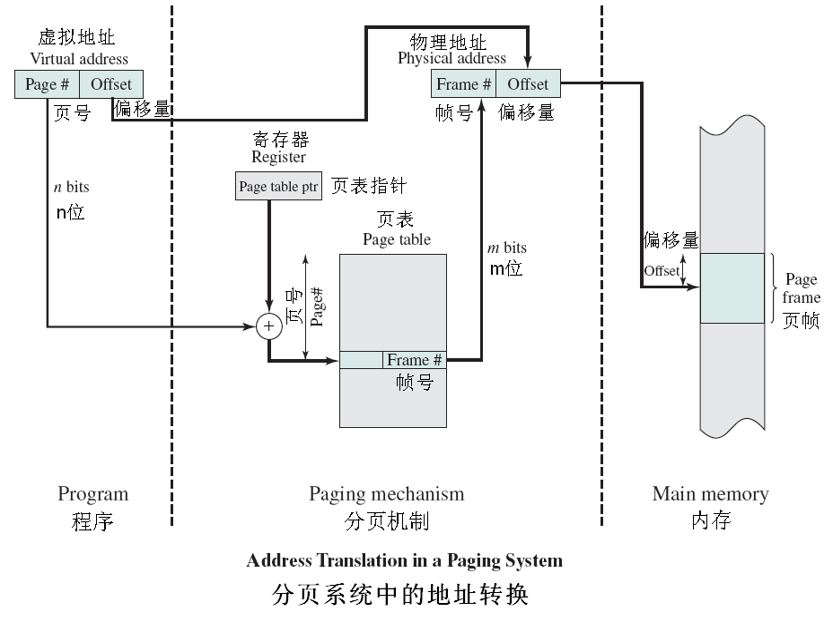
\includegraphics[width=0.8\linewidth]{fig/memory_address_transformation.png}
\end{figure}

\begin{figure}[H]
    \centering
    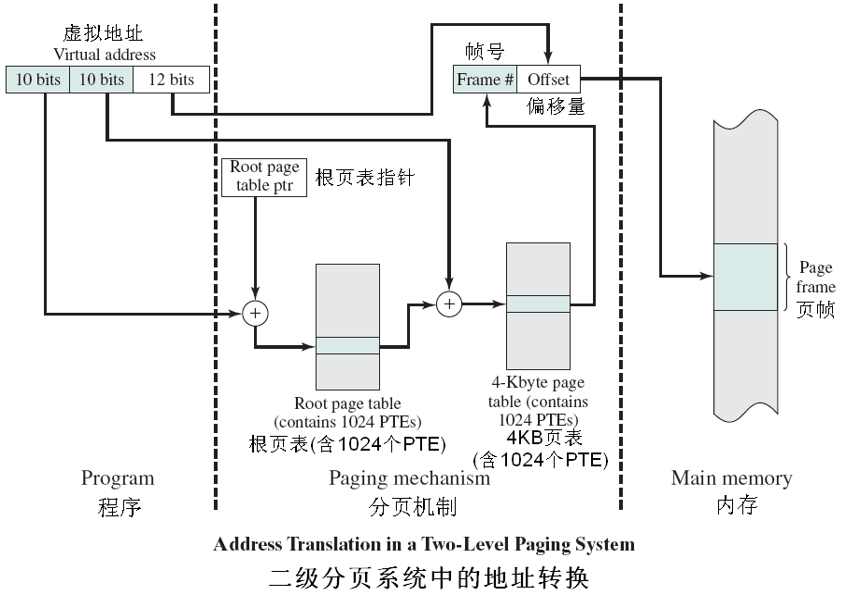
\includegraphics[width=0.8\linewidth]{fig/two-level_paging.png}
\end{figure}

快表/联想存储器(TLB)
\begin{figure}[H]
    \centering
    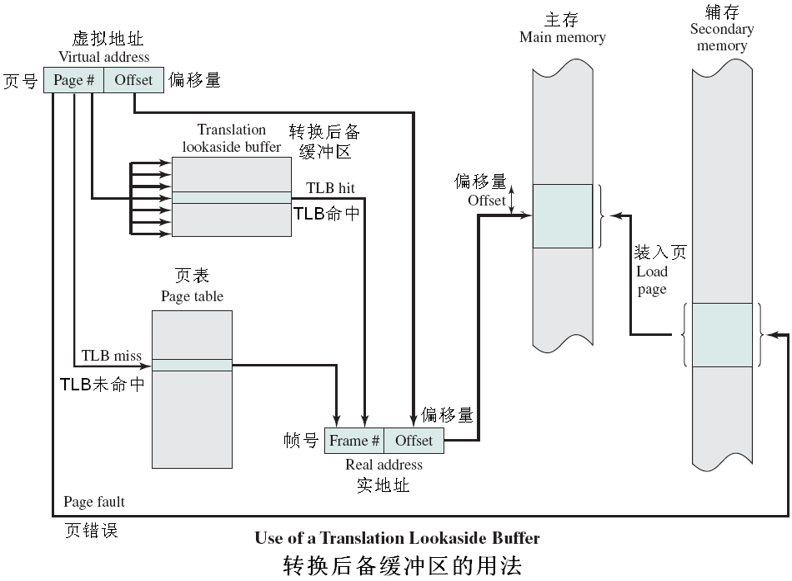
\includegraphics[width=0.8\linewidth]{fig/TLB.png}
\end{figure}

常见页面大小介于1KB-8KB

\begin{itemize}
    \item 调页策略:按需调页、预先调页
    \item 替换策略:
    \begin{itemize}
        \item Opt(Belady):置换下次访问距当前时间最长的页
        \item LRU:最近最少使用
        \item FIFO:先进先出
        \item Clock:时钟,需要附加位,首次/被置换放入置为1,顺序循环扫描页表,将1置0,并选择第一个原来就是0的页表项放置
    \end{itemize}
\end{itemize}

Linux的内存管理
\begin{itemize}
    \item 虚拟存储采用三级页表
    \item 页面分配采用伙伴系统
    \item 页面替换采用时钟算法
\end{itemize}